\documentclass[tikz,border=1.35mm]{standalone}

% Plain pentagonal face used in the FVMAdapt overview figures.
% Coordinates are in millimeters; y=-1mm keeps the SVG-style origin at top left.
\begin{document}
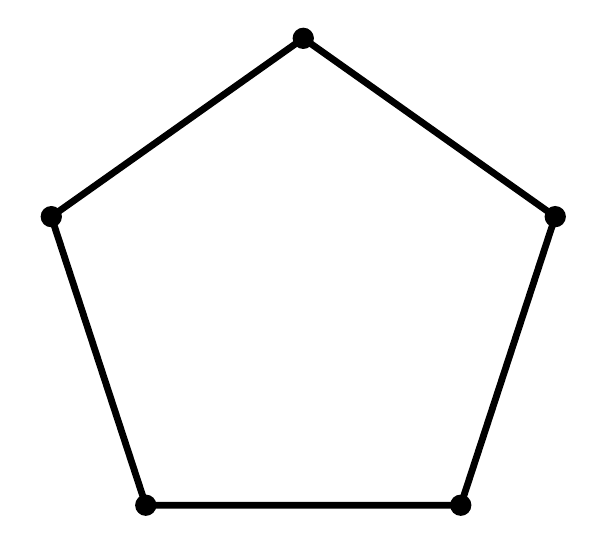
\begin{tikzpicture}[x=1mm,y=-1mm,line join=round]
  % Match the artwork frame before the standalone border is applied.
  \useasboundingbox (0,0) rectangle (70.000,62.000);

  % Pentagon vertices, ordered around the face.
  \coordinate (v0) at (35.000,1.353);
  \coordinate (v1) at (67.000,24.000);
  \coordinate (v2) at (55.000,60.647);
  \coordinate (v3) at (15.000,60.647);
  \coordinate (v4) at (3.000,24.000);

  % Draw edges first so vertex markers sit cleanly on top.
  \draw[line width=0.865mm] (v0) -- (v1) -- (v2) -- (v3) -- (v4) -- cycle;

  % Original vertices are black.
  \fill[black] (v0) circle[radius=1.353mm];
  \fill[black] (v1) circle[radius=1.353mm];
  \fill[black] (v2) circle[radius=1.353mm];
  \fill[black] (v3) circle[radius=1.353mm];
  \fill[black] (v4) circle[radius=1.353mm];
\end{tikzpicture}
\end{document}
